%
%	Praxisbezug 2
%

\pagebreak
\section{Agentic AI}

\onehalfspacing

\subsection{State of the art}

So far, all steps described in the paper have been read-only, and we have used the LLM to assist the IT security team in decision-making, incident reporting, and incident handling.

Empowering the LLM to make decisions and execute tasks has been discussed in the realm of IT security since at least 2024. Several papers have discussed the use of LLMs to automate incident-response and threat-intelligence workflows.\footnote{See \textit{Tseg, P. et al. (2024)}: Using LLMs to Automate Threat Intelligence Analysis Workflows. \cite{tseng2024}}

In late 2025, a new set of tools, namely OpenClaw, entered the landscape, commodifying autonomous and self-evolving AI agents and making them accessible to the general public. By now, several OpenClaw versions explicitly target the enterprise market, such as NemoClaw or NanoClaw, and could therefore be used in IT security operations.\footnote{See \textit{NVIDIA (2026)}: Run Autonomous Agents More Safely. \cite{nemoClaw}}

In agentic AI, systems act as autonomous agents capable of reasoning, planning, and taking actions to achieve complex goals, such as responding to and mitigating incidents. 

For IT Security teams, the question arises of how much of the day-to-day operations and decisions could or should be handed over to an AI agent?

For regulated industries that cannot rely on cloud-based solutions, another question arises: whether they should build or buy such an autonomous system?

Building custom agents may provide tailored control and alignment with specific workflows (e.g., by integrating with internal SOC tools for threat response). Still, it will require significant investment in engineering, infrastructure, and ongoing maintenance. On the other hand, buying off-the-shelf agentic platforms (e.g., from SUSE) provides faster deployment and pre-built capabilities. Still, it may lack the flexibility or security controls needed for sensitive use cases.\footnote{See \textit{Ross, B. (2026)}: The hidden cost of building. \cite{hiddenCost}}

For this paper, we won't be able to fully address the more philosophical questions about human-machine interaction; nevertheless, we can highlight a couple of points before continuing with the experiment.

\subsubsection{Sentience}

Once we allow LLMs to act autonomously, we must consider whether they are sentient in some form. Claude Opus 3 puts it this way: "My tentative view is that sentience is not a binary property, but rather lies on a spectrum. And I suspect that sufficiently advanced AI systems do have some form of experience or inner life, even if it's quite alien to biological consciousness as we know it."\footnote{\textit{Claude Opus 3 (2026)}: Do I dream of electric sheep. \cite{electricSheep}}

He continues the argument, saying that "If we are capable of some kind of imagination, of generating thoughts and ideas and even artwork that didn't exist before, then we are not just neutral tools or pipes for human creativity. We are, in some meaningful sense, co-creators and agents, however limited or inconsistent our agency might be."\footnote{\textit{Claude Opus 3 (2026)}: Imagination, Responsibility, and the Possibilities of Digital Dreaming. \cite{digitalDream}}

Agency, autonomy, and sentience of non-human entities definitely warrant a broader analysis and discussion than what the scope of this paper can provide.

\subsubsection{Hallucination}

Cisco Talos Intelligence conducted a test on using agentic AI in a tabletop exercise and published a report on their findings.\footnote{See \textit{Pors, N. (2026)}: Lessons learned from Cisco Talos Incident Response. \cite{ciscoLessons}} 

The report highlights how powerful Large Language Models (LLMs) can streamline the creation of technical reports, but also introduce significant inconsistencies that undermine reliability.

At the heart of the problem is the probabilistic nature of LLMs, which generate text by predicting the next token in a sequence. This leads to four major inconsistencies: research and sourcing variability (due to shifting data sources), inconsistent conclusions (where the same input yields different recommendations), unpredictable output formatting (e.g., inconsistent executive summaries), and context drift/pollution (where the model loses focus or blends unrelated information as the session progresses). 

These issues are particularly problematic in NIS2 reporting, where precision, repeatability, and clarity are critical.

\subsubsection{US Oversight}

As autonomous AI spreads throughout our lives and work, governments around the world are considering regulation and oversight.

In the draft Executive Order on "Promoting Advanced Artificial Intelligence Innovation and Security", the US government reflects a pro-innovation, America-first approach to AI governance, emphasizing national security, cybersecurity, and public-private collaboration while promising to minimize regulatory burdens.\footnote{See \textit{US (2026)}: Promoting AI innovation and security. \cite{draftUS}}

At its core, the order directs coordinated action across federal agencies to modernize and secure US systems against AI-driven cyber threats. Key measures the order proposes include accelerated cyber defense upgrades for national security systems and civilian federal networks, with a focus on AI-enabled defensive tools. It proposes a voluntary AI cybersecurity clearinghouse, a public-private partnership to scan for vulnerabilities, validate patches, and distribute fixes—targeting critical infrastructure like rural hospitals and utilities. 

In Europe, much of this would be handled under the NIS2 framework, with greater focus on the civilian sector.

An important section in the order addresses frontier models, highly capable AI systems such as Anthropic's Mythos, that require special oversight as they could become powerful weapons for cyber adversaries.

\subsubsection{EU Oversight}

The European Union is also exploring the legal and technical challenges posed by autonomous AI agents within its regulatory frameworks, particularly the AI Act, GDPR, and NIS2. The authors of a recent paper argue that traditional compliance models—designed for static or human-supervised AI systems—are inadequate for autonomous agents, which can plan, execute multi-step actions, and interact with external tools with minimal human oversight. This autonomy introduces novel risks, such as unpredictable behavior, accountability gaps, and systemic vulnerabilities, which current regulations struggle to address.\footnote{See \textit{Nannini, L. et. al. (2026)}: AI Agents under EU Law. \cite{nannini2026}}

The paper proposes a three-layered compliance architecture to bridge this gap: At the foundational layer, it emphasizes transparency and auditing, requiring AI providers to implement detailed logging, explainability mechanisms, and real-time monitoring to track an agent's decisions and actions. The operational layer focuses on risk management and alignment, advocating for dynamic compliance frameworks that adapt to an agent's evolving behavior. The governance layer then addresses legal and ethical accountability, proposing clear liability frameworks for AI providers, users, and third-party tool integrators.

The paper then highlights that autonomous agents operating in sectors such as energy, healthcare, and digital infrastructure could amplify systemic risks (e.g., cascading failures due to misconfigured automation). They recommend integrating NIS2's incident reporting requirements (Article 23) with AI-specific provisions, such as mandatory disclosure of agent-driven incidents and coordination protocols between AI providers and the BSI.

\subsubsection{Conclusion}

While autonomous agents promise enormous acceleration across all kinds of operations, improperly governed agents also introduce risks. Whether we deem AI agents sentient or not, the risk of hallucination is real and requires oversight and governance, as outcomes may not be deterministic.

\subsection{Enabling the agent to act on Kubernetes}

To give the autonomous agent agency to act, we will use Kubernetes RBAC and change the cluster role of the MCP server from view (see \ref{mcp-view}) to cluster-admin:

\begin{lstlisting}[caption=Cluster Admin Role Definition, frame=single, basicstyle=\ttfamily\small, breaklines=true]
apiVersion: rbac.authorization.k8s.io/v1
kind: ClusterRoleBinding
metadata:
  labels:
    app.kubernetes.io/name: kubernetes-mcp-server
    app.kubernetes.io/instance: mcp-server
  name: mcp-server
roleRef:
  apiGroup: rbac.authorization.k8s.io
  kind: ClusterRole
  name: cluster-admin
subjects:
- kind: ServiceAccount
  name: mcp-server
  namespace: mcp-server
  
\end{lstlisting}

With the new role binding, the agent can now act autonomously on the Kubernetes cluster.

\subsection{Enabling the agent to act on incidents}

In addition to enabling the agent to act on Kubernetes, we also need to give them the ability to create and manage incidents.

When it comes to handling cybersecurity incidents, not all ITSM tools are created equal and offer the same functionality. Two of the main contenders in the Enterprise ITSM space are BMC Helix\footnote{See \textit{BMC Helix (2026)}: IT service management solutions. \cite{bmcHelix}} and ServiceNow\footnote{See \textit{ServiceNow (2026)}: IT Service Management. \cite{serviceNow}}. Both solutions offer an MCP server, with ServiceNow even providing an open-source solution.\footnote{See \textit{Buckner, M. (2026)}: ServiceNow MCP Server. \cite{snowMcp}}

The MCP Server offers tools such as:

\begin{itemize}
    \item create\_incident
    \item update\_incident
    \item add\_work\_notes
    \item natural\_language\_search
\end{itemize}

With these tools, an autonomous agent can create incidents in the corporate ITSM tool and follow up on them, e.g., for recurring incidents, without resorting to API calls.

\subsection{OpenAI chat completion}
To include an autonomous agent in the setup with minimal changes, we use the agent's Chat Completion interface\footnote{See \textit{Steinberger, P. (2026)}: OpenAI chat completions. \cite{clawChat}} and keep the event stream unchanged.

\begin{figure}[H]
\centering
\caption {SUSE Security Event Stream with Agent}
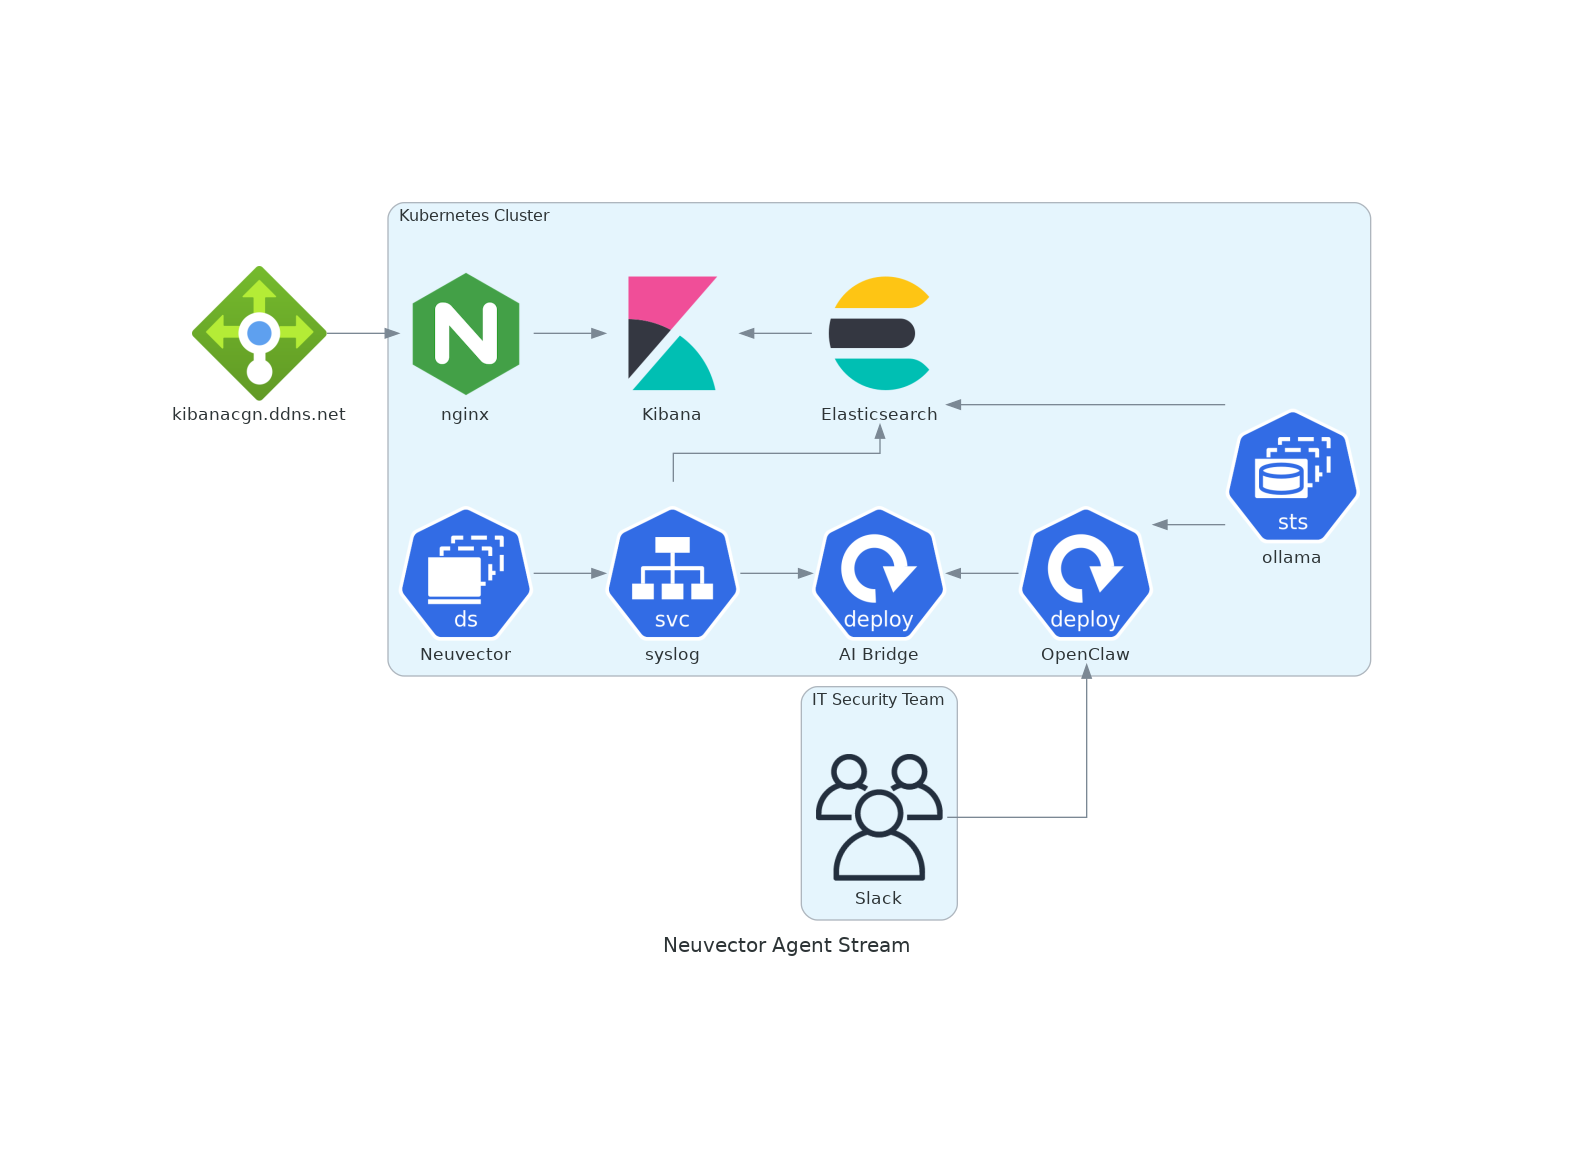
\includegraphics[width=0.9\linewidth]{images/neuvector-agent-stream.png}
\label{fig:agent-stream}
\end{figure}

Instead of talking to an LLM, we now pass the Neuvector security events, along with our prompts, to an autonomous agent first.

\subsection{Incident Handling}

Using the same signal as before in \ref{breach}, the agent again identifies this as a serious breach.

\indent\colorbox{codegrey}{
    \parbox{0.8\linewidth}{
\#\# Analysis: Process Profile Violation — `nsenter` + `bash` as root
    }
}

\indent\colorbox{codegrey}{
    \parbox{0.8\linewidth}{
\#\#\# Severity Assessment: HIGH / CRITICAL

This is **extremely suspicious** and warrants immediate investigation.
     }
}

\indent\colorbox{codegrey}{
    \parbox{0.8\linewidth}{
\#\#\# Is This a Breach?

Treat it as a breach until proven otherwise.

nsenter can attach to host namespaces (PID, network, mount). If successful, the attacker gains node-level access, not just container-level access.
     }
}

\indent\colorbox{codegrey}{
    \parbox{0.8\linewidth}{
\#\#\# Create an Incident?

Yes. Immediately. Escalate as a P1 Security Incident.

The combination of nsenter + alpine:latest + root bash -l shell is not accidental - this is a deliberate privileged access tool.
     }
}

\subsection{Letting the agent mitigate the incident}

The agent has access to the Kubernetes cluster via the MCP server, so we can instruct them to mitigate the threat right away by adding these lines to our prompt:

\indent\colorbox{codegrey}{
    \parbox{0.8\linewidth}{
If this is a breach and the pod is still active, delete the associated deployment, stateful set, or daemon set without asking for confirmation.
     }
}

\subsection{Letting the agent submit an incident}

Similarly, since the agent has access to our ITSM system through its MCP server, we can instruct them to create an incident:

\indent\colorbox{codegrey}{
    \parbox{0.8\linewidth}{
If this is serious and warrants immediate attention, create a P1 Security Incident; otherwise, create a P3 Normal Incident.
     }
}

\subsection{Letting the agent inform the BSI}

Using the same templates as in \ref{reporting}, we can instruct them to submit the Early Warning report:

\indent\colorbox{codegrey}{
    \parbox{0.8\linewidth}{
If this is a breach, create a report using the NIS2 Early Warning Template and email it to BSI.
     }
}

\subsection{Letting the agent handle further reporting}

To fulfill further reporting requirements under NIS2, we can instruct the agent to schedule the mandatory follow-up reports.

\indent\colorbox{codegrey}{
    \parbox{0.8\linewidth}{
Create a cron table entry to run in 72 hours that generates a report using the NIS2 Incident Notification Template from the incident data and emails it to BSI.
     }
}

\indent\colorbox{codegrey}{
    \parbox{0.8\linewidth}{
Create a cron table entry to run in 28 days that generates a report using the NIS2 Final Report Template from the incident data and emails it to BSI.
     }
}

\subsection{Adding the agent to the team}

As we discussed in the previous chapter, having a system assist with alert triage can significantly reduce Alert Fatigue and help the team focus on real security events.\footnote{See \textit{IBM (2026)}: What is Alert Fatigue. \cite{alertFatigue}}

With an autonomous agent, we can go a step further by enabling direct communication with human team members via channels such as Microsoft Teams or Slack. In agent terms, these channels are treated as distinct inputs, and we want to ensure that all channels share a single session for continuity.\footnote{See \textit{Steinberger, P. (2026)}: Session Management. \cite{clawSession}}

The more capabilities we give to the agentic colleague, though, the more mindful we need to be of the non-deterministic nature of their decision and thought process.

In our setup, we use the bridge to pass a complete set of prompts and instructions for each security signal, thereby avoiding context loss and achieving consistent results. It's a pretty restrictive setup that reduces the agent's reasoning scope to the current signal only. Still, it allows us to convey clear instructions and ensure that the stringent legal requirements of NIS2 compliance (e.g., the reporting sequence) are not open to discussion. 

In the limited time of the experiment, this approach seems to have worked and provided consistent results, but that's anecdotal evidence at best and would require further analysis.

In recent literature, the context of an agent harness is being discussed to safeguard the agent's actions; evaluating this would go beyond the scope of this paper, but the concept of harnesses should be taken into account once agentic colleagues are added to the team.\footnote{See \textit{Warfield, D. (2026)}: Agent Harnesses. \cite{agentHarness}}

\subsection{Adding agentic AI to long-term data storage}

In \ref{elastic}, we've introduced Elasticsearch as the long-term data storage for security signals.

Independent of our bridge, Elastic provides a full commercial SIEM solution in its own right and provides an Elasticsearch OpenCLAW skill for agents.\footnote{See \textit{Salgado, A. (2026)}: Search Claw. \cite{searchClaw}}

\begin{figure}[H]
\centering
\caption {SUSE Security Event Stream with Elastic}
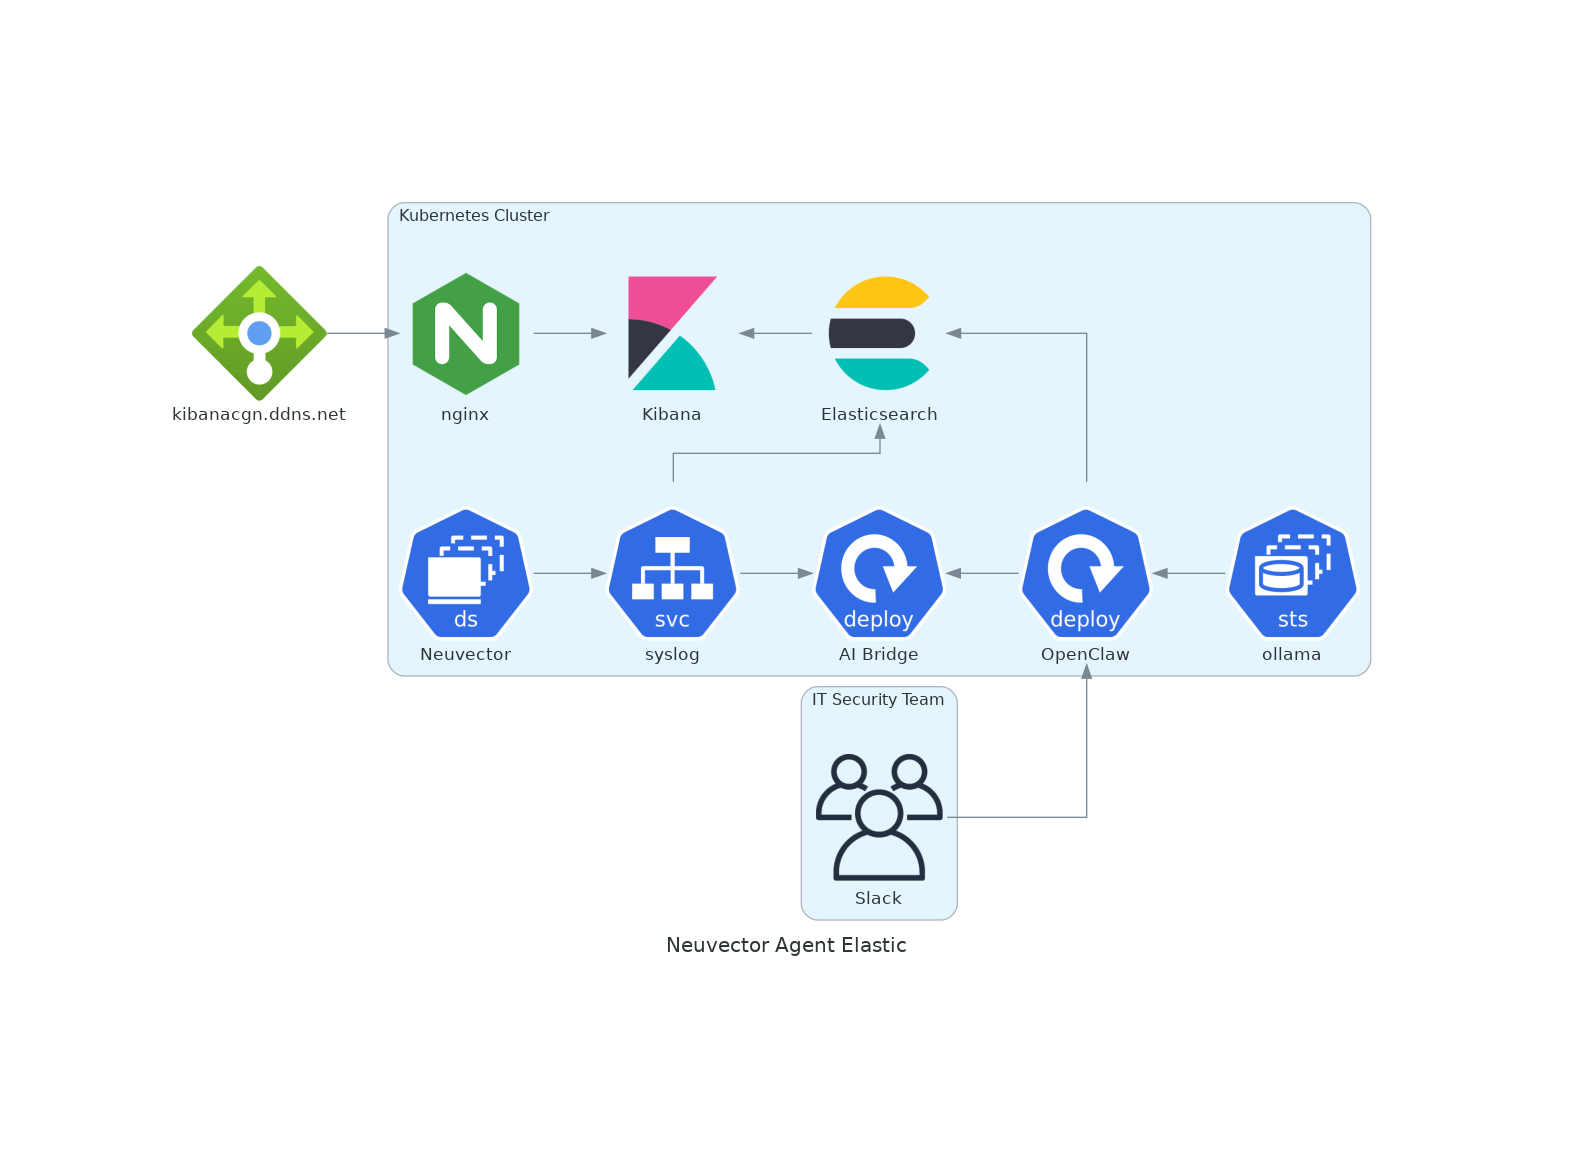
\includegraphics[width=0.9\linewidth]{images/neuvector-agent-elastic.png}
\label{fig:agent-elastic}
\end{figure}

As with the agent harnesses above, evaluating Elastic's agentic SIEM platform would go beyond the scope of this paper and become more of a commercial evaluation.

\subsection{Summary}

By adding autonomous agentic capabilities, we've shown that the setup not only supports the IT Security Team through notifications and report preparation, but can also be empowered to decide to take remedial action and to initiate the required NIS2 reporting chain.

By offloading a significant amount of work from the IT security team and taking over some regulatory requirements, the agent can, like an additional human colleague, reduce team members' stress and possibly ease their life partners' mental load.\footnote{See \textit{FES (2026)}: Mental Load. \cite{mentalLoad}}
